\documentclass[11pt,a4paper]{article}
\usepackage[utf8]{inputenc}
\usepackage{hyperref}
\usepackage{authblk}
\usepackage{color}
\usepackage{fullpage}

\usepackage{caption}

\usepackage{tikz}
\usetikzlibrary{bayesnet}
\usepackage{graphicx}
\usepackage{amsfonts}
\usepackage{amsmath,bm}
\usepackage{enumitem}
\usepackage[linesnumbered,ruled,vlined]{algorithm2e}

\usepackage{graphicx}
\graphicspath{ {./images/} }

\usepackage{minted}

\usepackage[backend=biber, style=nature, citestyle=nature]{biblatex}

\addbibresource{zotero_lib.bib} %Imports bibliography file

\renewcommand{\topfraction}{.85}
\renewcommand{\bottomfraction}{.7}
\renewcommand{\textfraction}{.15}
\renewcommand{\floatpagefraction}{.3}
\renewcommand{\dbltopfraction}{.3}
\renewcommand{\dblfloatpagefraction}{.3}
\setcounter{topnumber}{9}
\setcounter{bottomnumber}{9}
\setcounter{totalnumber}{20}
\setcounter{dbltopnumber}{9}

\usepackage{color}
\newcommand{\red}{\textcolor{red}}
\newcommand{\blue}{\textcolor{blue}}

\title{cell2location: high throughput spatial mapping of cell types and their interactions \\
Supplementary Methods
}

\author{Vitalii Kleshchevnikov, Emma Dann, Alexander Aivazidis, Artem Shmatko, Artem Lomakin, Mika Sarkin Jain, Liz Tuck, Anna Arutyunyan, Lauma Ramona, Kirsty Ambridge, Monika Dabrowska, Moritz Gerstung, Oliver Stegle, Omer Bayraktar}
\date{March 2020}

\begin{document}

\maketitle

\tableofcontents

\section{Mapping cell types with cell2location model}

\subsection{Cell2location model} \label{cell2location_model}

Cell2location is a Bayesian model that is aimed at decomposing spot-level expression levels into a set of pre-defined reference programs. Graphical model is illustrated in Fig \ref{fig:graphical_model}. The input data of the method are as follows: \newline

Let $D=\{d_{s,g}\}$ be a $S \times G$ Spatial expression count matrix for locations $s=\{1..S\}$ and genes $g=\{1..G\}$. 
This matrix can be directly obtained from the 10X SpaceRanger software (see Section \ref{c2l_sp_proc}). \newline

Let $G=\{g_{f,g}\}$, denote an $F \times G$ matrix of regulatory programs, which consist of $f=\{1..F\}$ reference programs with gene expression programs $g=\{1...G\}$. This matrix needs to be estimated from parallel scRNA-seq profiles. Strategies how to estimate this matrix are presented in Section~\ref{c2l_ref_prog}. \newline

Cell2location models the elements of $D$ as Poisson distributed, given an unobserved rate $\mu$ and a gene-specific over-dispersion parameter $\alpha_g$ which describes variance in expression of individual genes that is not unexplained by the regulatory programs: 
\begin{equation} \label{eq:c2l:1}
D_{s,g} \sim \mathtt{NB}(\mu^{fact}_{s,g}, \alpha_g) \\
\end{equation}

Note that this is equivalent to a Poisson variable (measurement model) with a Gamma-distributed mean (expression model \textsuperscript{\cite{sarkar_separating_2020}}).
\begin{equation} \label{eq:c2l:1}
D_{s,g} \sim \mathtt{Poisson}(\mathtt{Gamma}(\alpha_g, \alpha_g / \mu^{fact}_{s,g})) \\
\end{equation}

The spatial expression levels of genes $\mu^{fact}_{s,g}$ in the rate space are modelled as the sum of five non-negative components:
\begin{equation} \label{eq:c2l:3}
\mu^{fact}_{s,g} = m_{g} \left (\sum_{f} {w_{s,f} \: g_{f,g}} \right) + l_s + s_{g}\\
\end{equation}

Here, $w_{s,f}$ denotes regression weight of each program $f$ at location $s$ 
\red{would drop this here:
representing a combination of cell number, the fraction of each cell cytoplasm captured and cell-cell heterogeneity in expression}; 
$m_{g}$ denotes a gene-specific scaling parameter which accounts for difference in the global expression estimates between technologies;
$l_{s}$ and $s_{g}$ are additive components that capture background variation that is not explained by the bi-variate decomposition;
\red{ already defined:
$g_{fg}$ denotes expression signatures derived from single cell reference data.}


\red{again, think about better variable names.. this really messy}
The prior distribution on the unobserved parameters are as follows:
\begin{enumerate}
    \item The regression weights $w_{s,f}$ for each regulatory program are in turn Gamma distributed (Eq. \ref{eq:c2l:4} - \ref{eq:c2l:11}); and referred to in the package as \mintinline{python}|'spot_factors'|. \newline
    \begin{equation} \label{eq:c2l:4}
    w_{sf} \sim \mathtt{Gamma}({\mu}^{w}_{sf}, {\mu}^{w}_{sf} / c^{w})
    \end{equation}
    \red{add motivation, another decomposition to account for spatial correlation of programs across proximal spots}
    The mean ${\mu}^{W}_{sf}$ parameter is factorised into the latent positive spatial factor combinations $r$ to account for correlations in spatial expression of reference programmes $f$. The constant $c$ is used to control how informative the co-expression prior is.
    \red{define the number of r=1...R}
    \begin{equation} \label{eq:c2l:5}
    {\mu}^{W}_{sf} = (\sum_{r} {z_{sr} \: x_{rf}})\\
    \end{equation}
    
    \begin{itemize}
        \item The spatial location $z_{sr}$ of factor combinations $r$ across locations $s$ is defined as Gamma distributed
        \begin{equation} \label{eq:c2l:6}
        z_{sr} \sim \mathtt{Gamma}(N_s^{comb} / N^r, 1 / (N_s^{cells} / N_s^{comb}))
        \end{equation}
    
        The rate of $z_{sr}$ is defined as the inverse of the average number of cells in each location ($N_s^{cells}$) divided by the prior belief on the number of factor combinations $r$ $N_s^{comb}$ expressed in each location $s$. \newline
        Shape parameter of $z_{sr}$ accounts for the sparsity and is equal to the ratio of the number of factor combinations $N_s^{comb}$ present in each location $s$ to the total number of combinations $N^r$ (specified by the user, default is 50). This formulation specifies the prior on $z_{sr}$ such that $\sum_{f} z_{sr} = E(N_s^{cells})$ on average equals to the number of cells per location, and that on average each location contains substantial weights for $N^{comb}$ / $N^f$ combinations. \newline
        $N_s^{comb}$ and $N_s^{cells}$ are modelled as unobserved Gamma-distributed variables whose prior depends on prior knowledge about the tissue used to produce spatial data $D_{sg}$. So, the model does not require knowing the exact number of cells obtained by counting nuclei in each spot. User needs to provide rough estimate of the average number of cells $N^{cells-mean}$ and co-located cell combinations in the tissue $N^{comb-mean}$, as well as provide a measure of uncertainty $v$ in that estimate in eq \ref{eq:c2l:7} - \ref{eq:c2l:8}. \newline
        \begin{equation} \label{eq:c2l:7}
        N_s^{comb} \sim \mathtt{Gamma}(N^{comb-mean}, N^{comb-mean} / v^{comb})
        \end{equation}
        \begin{equation} \label{eq:c2l:8}
        N_s^{cells} \sim \mathtt{Gamma}(N^{cells-mean}, N^{cells-mean} / v^{cells})
        \end{equation}
        Nonetheless, if segmentation data for each location is available it can be provided as a location-specific $N_s^{cells-mean}$ prior.
        
        \item The latent variable $x_{rf}$ representing the contribution of each factor $f$ to combinations $r$ is modelled as Gamma distributed with a hierarchical prior $N_r^{f-per-r}$ on the number of factors $f$ non-zero in each combination $r$:
        \begin{equation} \label{eq:c2l:10}
        x_{rf} \sim \mathtt{Gamma}(N_r^{f-per-r} / N^r, N_r^{f-per-r})
        \end{equation}
    
        $N_r^{f-per-r}$ is also unobserved and Gamma-distributed with an informed prior on the number of co-located factors $N^{f-per-r-mean}$ and a measure of uncertainty in that prior $v$:
        \begin{equation} \label{eq:c2l:11}
        N_r^{f-per-r} \sim \mathtt{Gamma}(N^{f-per-r-mean}, N^{f-per-r-mean} / v^{f-per-r-mean})
        \end{equation}
        where high values of $N^{f-per-r-mean}$ indicate that each factor $f$ is co-located with many others, and $N^{f-per-r-mean} = 1$ indicates that the spatial profile of each factor $f$ is independent from the rest. Under this prior $E(\sum_{f} z_{sr}) = 1$ which gives ${\mu}^{W}_{sf}$ absolute scale of the number of cells per locations $s$ expressing each factor $f$.
    
        \end{itemize}
    
    \item $m_{g}$ is modelled as Gamma-distributed (Eq. \ref{eq:c2l:12} - \ref{eq:c2l:14}) with hierarchical prior $\alpha^M$ and $\beta^M$ reflecting the prior belief about the difference in sensitivity of single cell and spatial technologies. Specifically average change in sensitivity $\mu$, the extent to which individual genes deviate from $\mu$ ($\sigma$) and our uncertainty in these priors $z$ (expressed as mean / variance ratio).
    \begin{equation} \label{eq:c2l:12}
    m_{g} \sim \mathtt{Gamma}(\alpha^m, \beta^m) 
    \end{equation}
    \begin{equation} \label{eq:c2l:13}
    \alpha^m \sim \mathtt{Gamma}(\mu ^ 2 / \sigma ^ 2,  \sqrt{\mu ^ 2 / \sigma ^ 2 / z})
    \end{equation}
    \begin{equation} \label{eq:c2l:14}
    \beta^m \sim \mathtt{Gamma}(\mu / \sigma ^ 2,  \sqrt{\mu / \sigma ^ 2 / z})
    \end{equation}
    
    $\mu ^ 2 / \sigma ^ 2$ converts our guess of the average change in sensitivity $\mu$ into the mean of the shape parameter of $\alpha^M$. This way we are not forcing change in sensitivity $\mu$ but allowing the model to learn it. Rate of Gamma distribution $\beta^M$ is defined according to Eq. \ref{eq:c2l:14}.
    
    \item $l_s$ and $s_{g}$ are modelled as Gamma distributed with hierarchical priors on shape and rate of their distributions eq. \ref{eq:c2l:15} - \ref{eq:c2l:20}:
    \begin{equation} \label{eq:c2l:15}
    l_s \sim \mathtt{Gamma}(\alpha^l,  \beta^l)
    \end{equation}
    \begin{equation} \label{eq:c2l:16}
    \alpha^l \sim \mathtt{Gamma}(1, 1)
    \end{equation}
    \begin{equation} \label{eq:c2l:17}
    \beta^l \sim \mathtt{Gamma}(1, 1)
    \end{equation}
    
    \begin{equation} \label{eq:c2l:18}
    s_{g} \sim \mathtt{Gamma}(\alpha^s,  \beta^s)
    \end{equation}
    \begin{equation} \label{eq:c2l:19}
    \alpha^s \sim \mathtt{Gamma}(1, 1)
    \end{equation}
    \begin{equation} \label{eq:c2l:20}
    \beta^s \sim \mathtt{Gamma}(1, 1)
    \end{equation}
    
    \item Containment prior is used for modelling unobserved variance using NB overdispersion $\alpha_g$ \textsuperscript{\cite{simpson_penalising_2017}}. Under the following prior most genes have low overdispersion:
    \begin{equation} \label{eq:c2l:21}
    \alpha_g = 1 / o_g ^ 2
    \end{equation}
    \begin{equation} \label{eq:c2l:22}
    o_g \sim \mathtt{Exponential}(\mu^o)
    \end{equation}
    \begin{equation} \label{eq:c2l:23}
    \mu^o \sim \mathtt{Gamma}(mu,  sd)
    \end{equation}
    Constants $mu$ and $sd$ parameterising Gamma distribution in eq \ref{eq:c2l:23} are chosen to appropriately scale the exponential distribution in eq \ref{eq:c2l:22}. The inference of this parameter appears to be fairly robust to the choice of $mu$ and $sd$.

\end{enumerate}


To give the inferred cell location parameters a physical meaning we compute the number of mRNA molecules ($u_{sf}$) contributed by each cell state $f$ to each location $s$:
\begin{equation} \label{eq:c2l:24}
u_{sf} = w_{sf} (\sum_{g} {m_{g} \: g_{fg}})
\end{equation}
These parameters are referred to in the package as \mintinline{python}|'nUMI_factors'|. \newline

\begin{figure}
    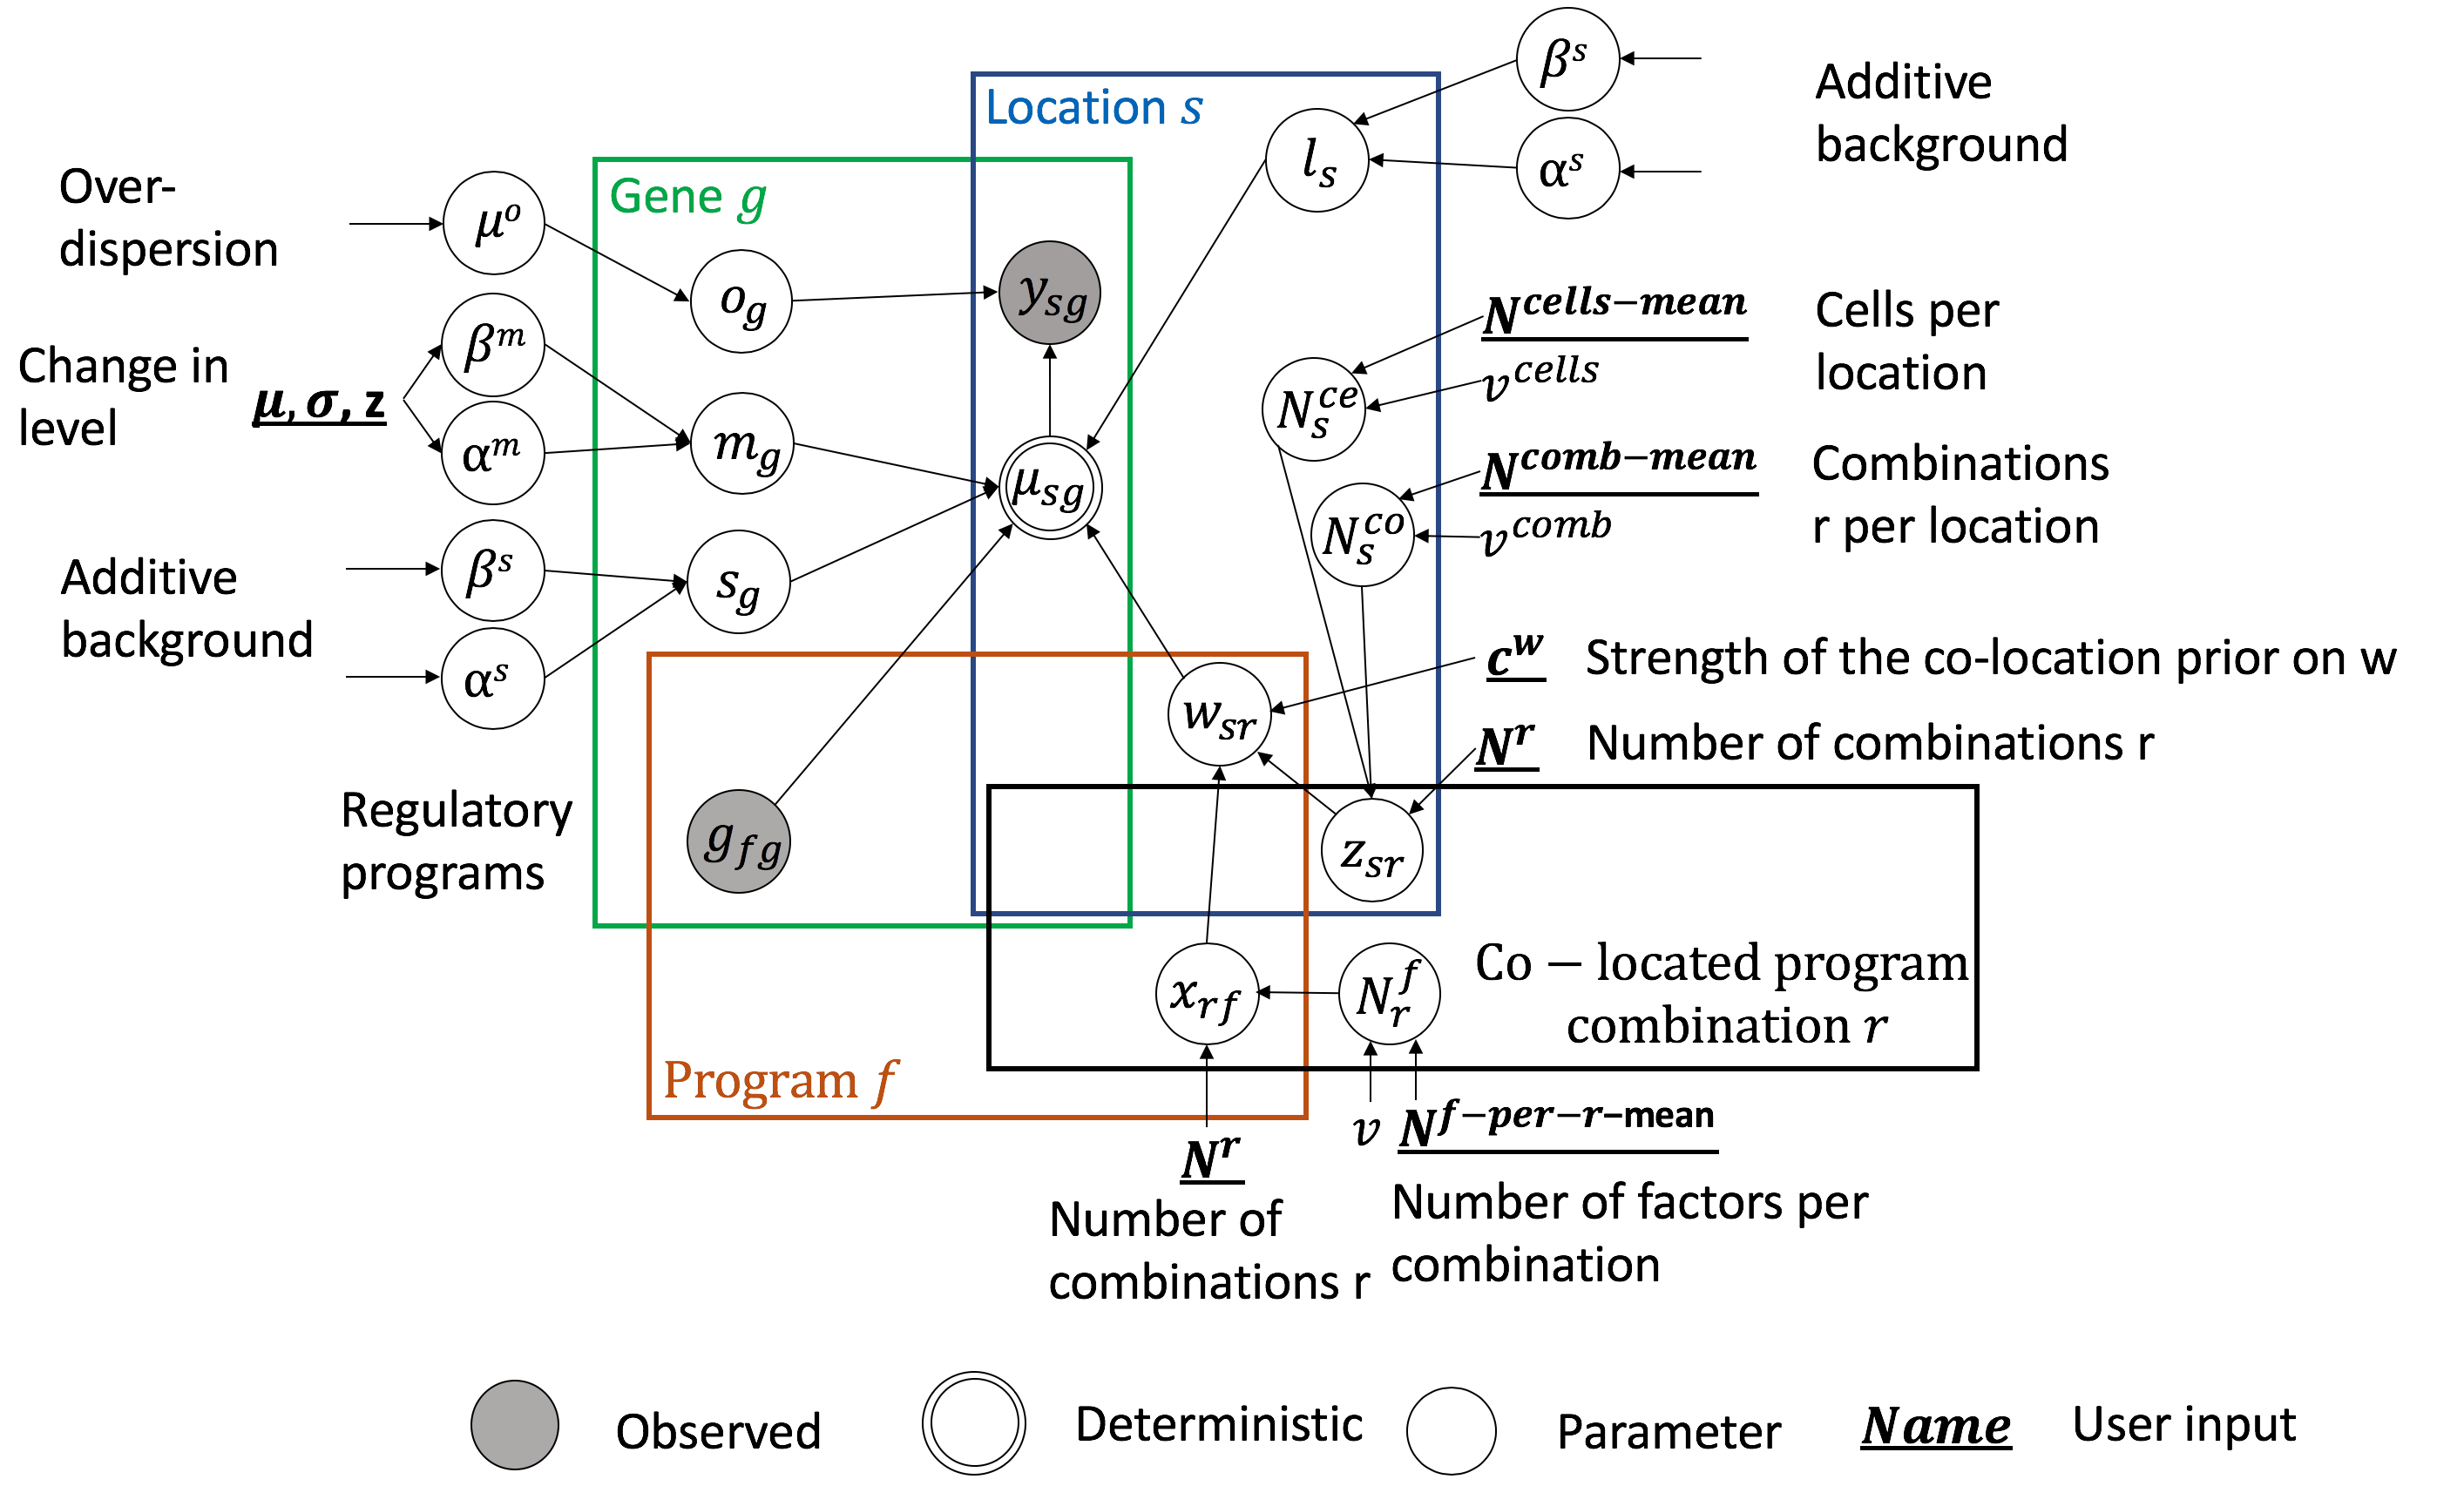
\includegraphics[scale=0.35]{images/CoLocationModelNB4V2.png}
    \caption{Illustration of the corresponding graphical model.}
    \label{fig:graphical_model}
\end{figure}

\subsection{Inference} \label{c2l_inference}

Variational Bayesian Inference is used to approximate the posterior, specifically black-box Automatic Differentiation Variational Inference (ADVI) implemented in pymc3 framework \textsuperscript{\cite{salvatier_probabilistic_2016}}. Appropriately transformed univatiate normal distribution is used to approximate each parameter. Inference is achieved by maximising log-likehood of the data and minimising KL divergence from the posterior to prior (ELBO loss function).
Several restarts are performed to evaluate the stability of the inferred posterior distribution. Under default parameters inference is very stable so no selection of the best model is performed (the first training restart is used). Validity of selected hyper-parameters is evaluated using prior predictive check. Performance of the training is evaluated by performing the posterior predictive check for the accuracy of the model at reconstructing expression levels of each gene $g$ in each location $s$; and by evaluating consistency of inferred $w_{sf}$ parameters between the training restarts.

- methods but also criteria\
- how many restarts, selection of “best” model, etc. 

\subsection{Processing of the spatial expression matrix} \label{c2l_sp_proc}
Expression $D_sg$ counts of each gene $g$ in each location $s$ are obtained from 10X Spaceranger 1.0.0. Untransformed and unnormalised count matrix was filtered to include genes expressed in the single cell reference $g_fg$ and used as input to the model.

\red{would call this estimation of programs..}
\subsection{Derivation of reference expression programs} \label{c2l_ref_prog}a
\red{the matrix $D$ is used twice now. I would use a different variable name... for spatial and non-spatial data}
We obtain reference expression programmes $G$ from scRNA-seq reference expression data $D_cg$ of each gene $g$ in each cell $c$. Untransformed and unnormalised count matrix $D_cg$ is filtered to select expressed genes (at least 10 cells per gene). Using matched scRNA-seq profiles allows to know exactly which cells express which genes in the spatial sample. Using unmatched reference instead infers the location of the most similar regulatory program. We use following 2 alternative methods to compute $g_fg$:
\begin{enumerate}
    \item Analytically computing single cell reference cluster centroids for each gene $g$ and cell cluster $z$. This method is very computationally efficient and gives very good mapping quality (measured on simulated data) when the scRNA-seq reference is a single sample or a few samples matching the source of spatial data $D_{sg}$ with no strong batch effect between them.
    \item To address the usage of challenging reference data composed of multiple batches the expression of each gene $g$ in each single cell reference cluster $z$ is inferred using Negative Binomial regression. The model accounts for the sequencing coverage $h_e$ and background expression $g_{eg}$ in each sample $e$, and models unexplained variance (overdispersion $\alpha_g$) and count nature of the data using Negative Binomial distribution:
    \begin{equation} \label{eq:c2l_ref_prog:1}
    D_{cg} \sim \mathtt{NB}(\mu_{cg}, \alpha_g)
    \end{equation}
    \begin{equation} \label{eq:c2l_ref_prog:2}
    \mu_{cg} = (g_{zg} + g_{eg}) * {h_e}
    \end{equation}
    All model parameters are constrained to be positive to simplify interpretation. Weak L2 regularisation of $g_{zg}$ / $g_{eg}$ and penalty for large deviations of $h_e$ from 1 is used. $g_{zg}$ is initialised at analytical cluster centroids and $g_{eg}$ is initialised at average expression of each gene $g$ in each sample $e$ divided by a factor of 10. This leads to fast convergence, while pytorch implementation of training using minibatches makes model scalable to more than 100k cells and fast (30sec-5min on GPU). Maximum a posterior optimisation is used to find parameters of this model with batch size of 1024 cells, ADAM learning rate 0.01. The number of epochs needed for training is determined using cross-validation performed on held-out 10 percent of cells. \newline
    To verify that the model successfully accounted to non-biological sample effect we use $h_e$ and $g_{eg}$ to correct the expression matrix, followed by standard scanpy workflow \textsuperscript{\cite{wolf_scanpy_2018}} to verify the mixing of the cells from matching cells types but different samples:
    \begin{equation} \label{eq:c2l_ref_prog:3}
    D^{corrected}_{cg} = D_{cg} * {h_e} - g_{eg}
    \end{equation}

\end{enumerate}

\section{Clustering of tissue regions and diffusion maps of cell type gradients} \label{auto_clustering}

The cell density $w_{sf}$ (eq. \ref{eq:c2l:4}) inferred by cell2location model serves as a proxy to cell density. This enables describing similarity of locations (spots) by constructing a KNN graph that represents connectivity of locations in terms of their in cell composition (N neighbours = 20 for human lymph node, 38 for the mouse brain). Standard implementation of Leiden clustering and diffusion maps \textsuperscript{\cite{wolf_scanpy_2018}} can utilise cell composition KNN graph to characterise organisation of the tissue. We used both methods with default arguments (resolution parameter of Leiden clustering = 1). Obtained regions were cross-referenced with the mouse brain anatomy using corresponding histology images and similar clusters were merged to generate the broad region map.

\section{Cellular interaction neighbourhoods of co-located cell types} \label{cell_neighbourhoods}

To map out cellular interaction neighbourhoods we combined de-novo non-negative matrix factorisation model with receptor-ligand analysis using CellPhoneDB \textsuperscript{\cite{vento-tormo_single-cell_2018}}. We used hierarchical Poisson matrix factorisation model to simultaneously infer combinations of co-located regulatory programmes and where in the tissue they locate. We assume that correlation in density of cell types across locations reflects the interaction between these cell types, specifically, any interaction that could affect mutual location of these cell types:
\begin{itemize}
    \item Signals promoting proliferation and survival of other cell type
    \item Adhesion molecules that increase the frequency of contacts 
    \item Recruitment signals such as CXCR5 / CXCL13 \textsuperscript{\cite{van_de_pavert_chemokine_2009}}
    \item Repulsive signals, inhibiting the action of chemotaxis signals such as PD-1 / PD-L1 interactions \textsuperscript{\cite{shi_pd-1_2018}}
    \item Interactions that induce new transcriptional states 
\end{itemize}

Visium technology serves as a native binning strategy to identify regions of action for local paracrine signals (within the $55\mu m$ spot diameter). We assume that the signal does not propagate between neighbouring spots spaced by $45\mu m$ gaps.

Therefore our Poisson factorisation model reveals which cell types interact with consequences to their location and where these interactions occur. 

To find a small number of co-located combinations representing the broad grouping of cell types - a few factors were selected. This has the advantage of identifying overlapping but distinct combinations compared to Leiden clustering.
To find very strong co-location signal, assuming that most cell types (regulatory programmes) are independent, a lot of factors were used (e.g. 32).

Inference is performed using standard NMF in the scikit-learn \textsuperscript{\cite{scikit-learn}}.

\subsection{Description of the co-located combination model} \label{cell_neighbourhoods_model}

Density $w_{sf}$ of each cell type $f$ across locations $s$ is modelled as an additive function of cell neighbourhoods $r$. This means the density of one cell type in one location can be explained by 2 distinct combinations $r$. Cell type density is therefore a function of the following non-negative components:  
\begin{equation} \label{eq:circ:1}
w_{sf} = (\sum_{r} {i_{sr} \: k_{rf} \: m_{f}})
\end{equation}

\begin{enumerate}
    \item $k_{rf}$ represents the proportion of cells of each type (regulatory programmes) $f$ that correspond to each co-located combination $r$, normalised for total abundance of each cell type $m_{f}$.
    \item $m_{f}$ cell type budget accounts for the difference in abundance between cell types, thus focusing the interpretation of $k_{rf}$ on cell co-location.
    \item $i_{sr}$ is proportional to the number of cells from each neighbourhood $r$ in each location $s$, and shows the abundance of combinations $r$ in locations $s$.
\end{enumerate}

In practice $q_{rf} = k_{rf} \: m_{f}$ is obtained from scikit-learn NMF and normalised by the sum across factors to obtain $k_{rf}$:
\begin{equation} \label{eq:circ:2}
k_{rf} = q_{rf} / (\sum_{r} q_{rf})
\end{equation}

\section{References}

\printbibliography

\end{document}